\newpage
\section{Test 8}
\label{Sec:test_8}

In the eighth test setting rover is placed on the surface of an inclined plane. Inclination angle of the slope has been set to 10$^\circ$. After initial period equal torques are applied to all wheels causing rover to move in circle. To carry out circular motion rover's wheels have been oriented as follows:

\begin{itemize} 
  \item Front left wheel $\gamma = 0.407rad$           
  \item Front right wheel $\gamma = 0.107rad$        
  \item Middle left wheel $\gamma = 0rad$           
  \item Middle right wheel $\gamma = 0rad$        
  \item Rear left wheel $\gamma = -0.407rad$           
  \item Rear right wheel $\gamma = -0.107rad$        
\end{itemize}

\noindent In order to retain the initial orientation of the steering axis PD controller has been incorporated into rover's dynamics. 

\begin{figure}[H]
  \centering
    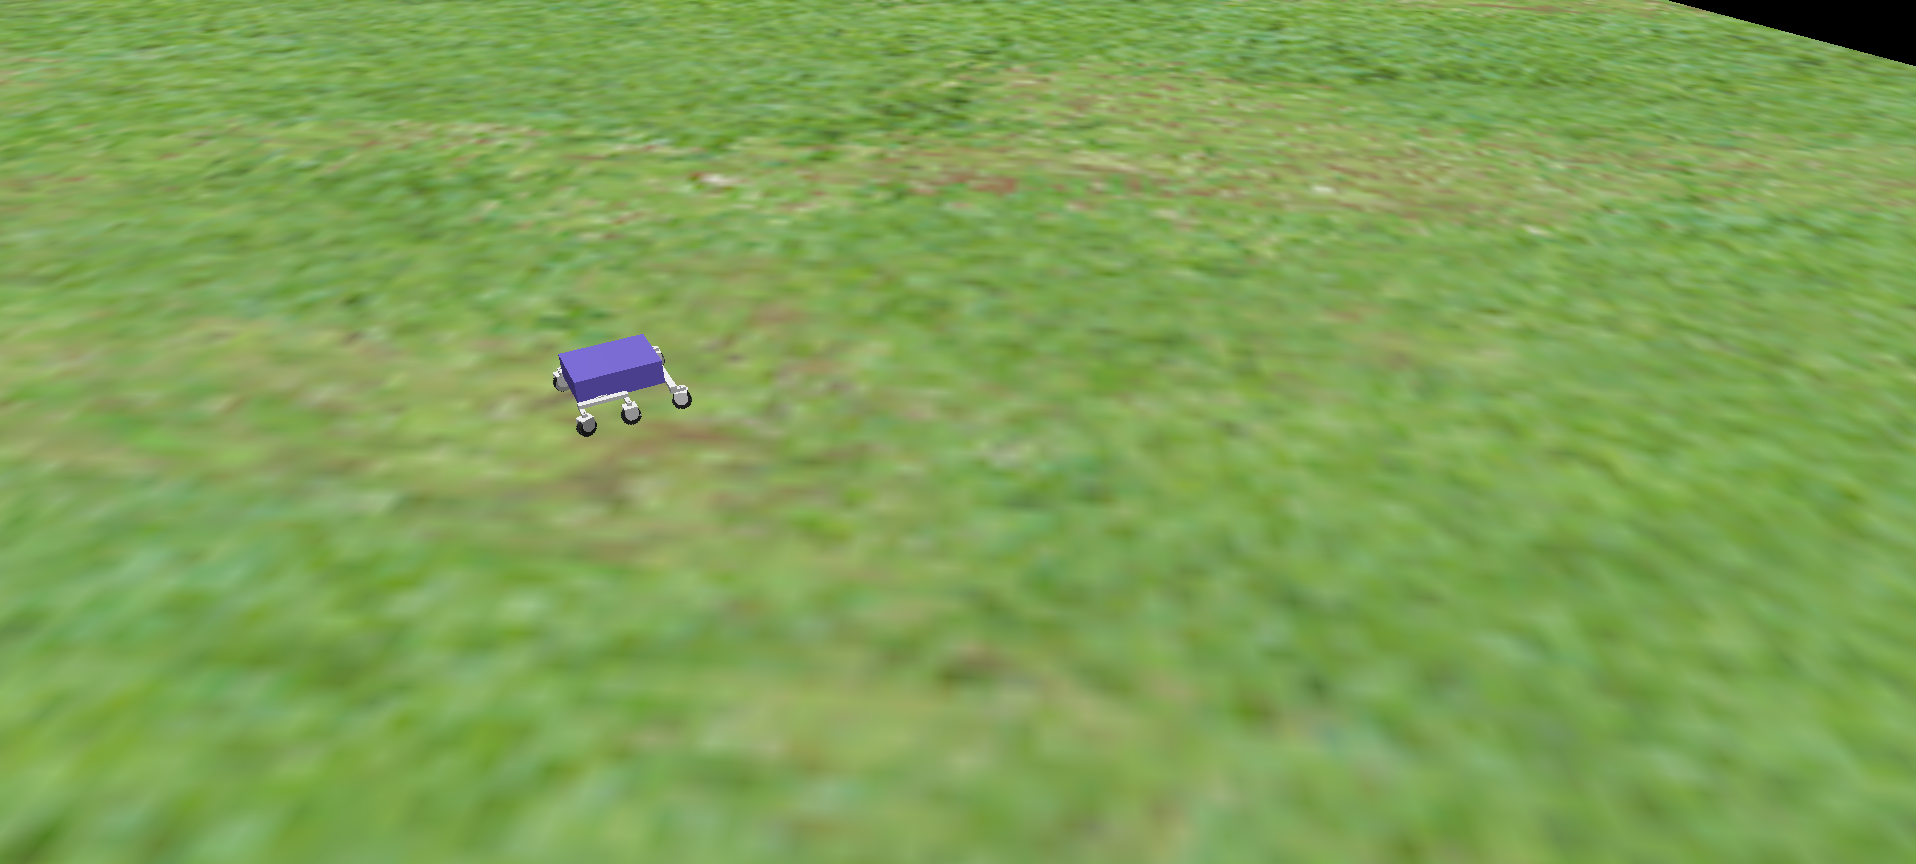
\includegraphics[width=0.8\textwidth]{run_8}
  \caption{Eighth test scenario}
\end{figure}

\noindent In this case, following quantities have been plotted:

\begin{itemize}
  \item $x_{COM}$ - mass center coordinates
\end{itemize}

\begin{figure}[H]
  \centering
    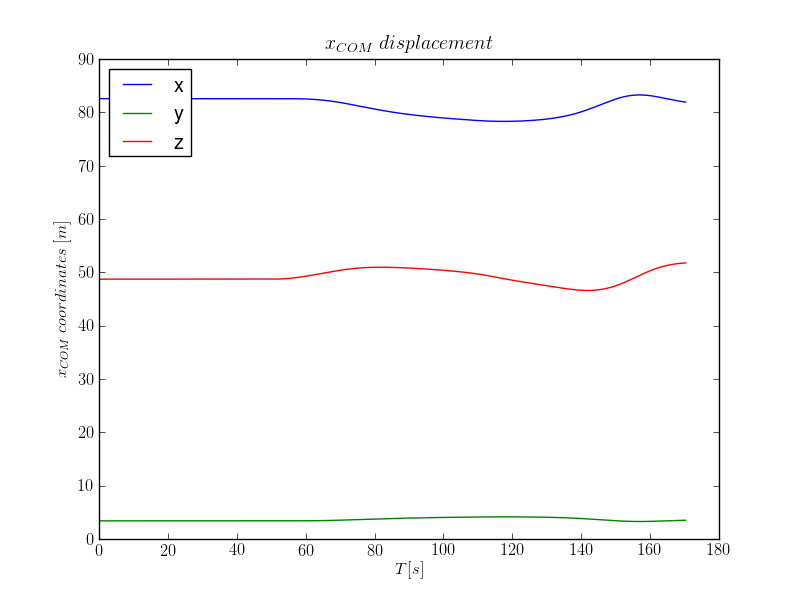
\includegraphics[width=0.8\textwidth]{xCOM8}
  \caption{$x_{COM}$}
\end{figure}

\begin{itemize}
  \item $x_{wheels}$ - wheels angular displacement 
\end{itemize}

\begin{figure}[H]
  \centering
    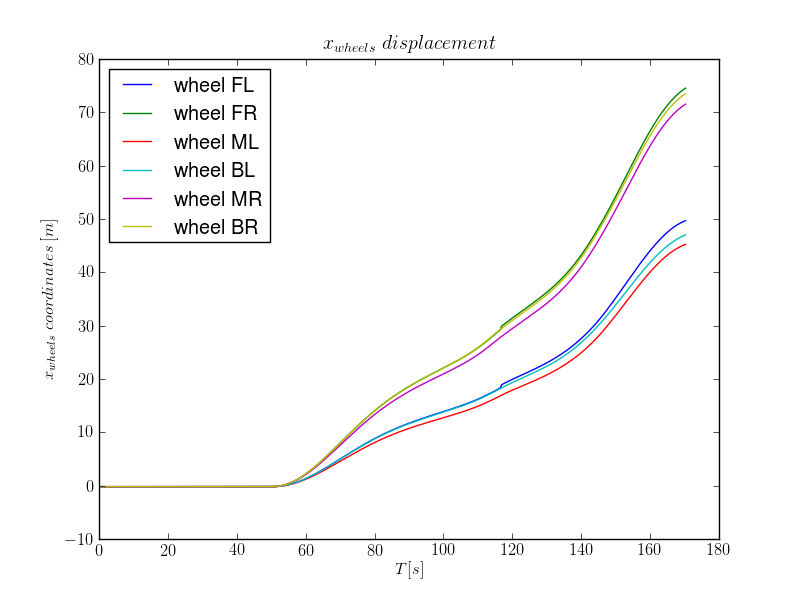
\includegraphics[width=0.8\textwidth]{xWHEELS8}
  \caption{$x_{wheels}$}
\end{figure}

\begin{itemize}
  \item $v_{COM}$ - mass center velocity
\end{itemize}

\begin{figure}[H]
  \centering
    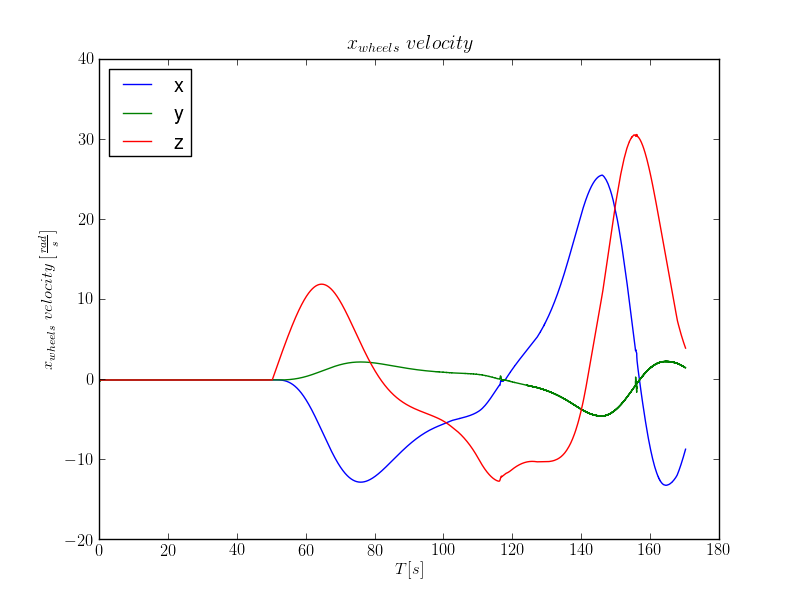
\includegraphics[width=0.8\textwidth]{vCOM8}
  \caption{$v_{COM}$}
\end{figure}

\begin{itemize}
  \item $R_{COM}$ - reaction forces of center of mass in lagrangian coordinates
\end{itemize}

\begin{figure}[H]
  \centering
    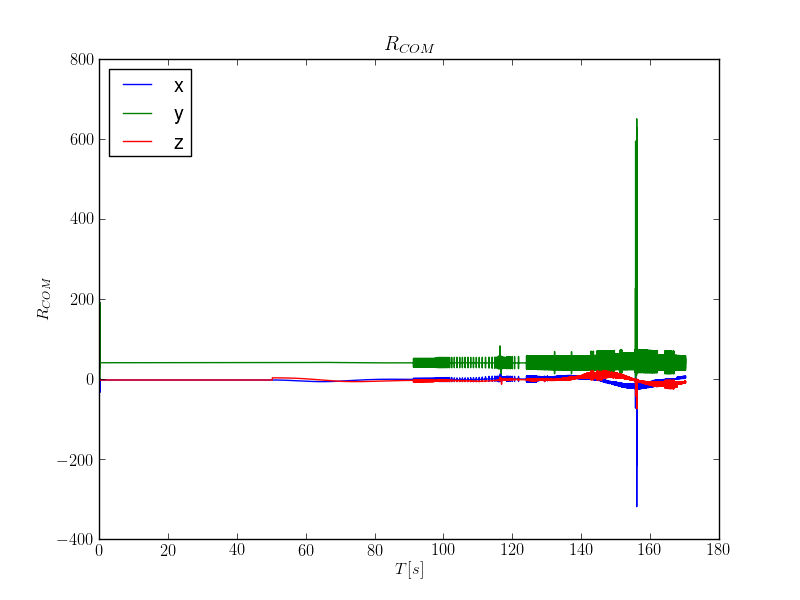
\includegraphics[width=0.8\textwidth]{pCOM8}
  \caption{$R_{COM}$}
\end{figure}

\begin{itemize}
  \item $R_{wheels}$ - reaction forces of wheels in lagrangian coordinates
\end{itemize}

\begin{figure}[H]
  \centering
    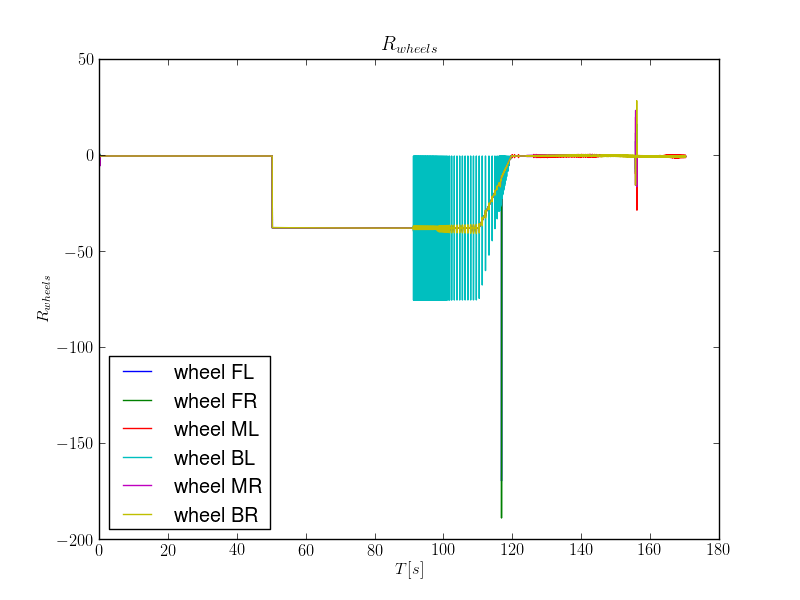
\includegraphics[width=0.8\textwidth]{pWHEELS8}
  \caption{$R_{wheels}$}
\end{figure}

\begin{itemize}
  \item $\lambda_{N}$ - normal component of the contact force (impulsion) for each wheel
\end{itemize}

\begin{figure}[H]
  \centering
    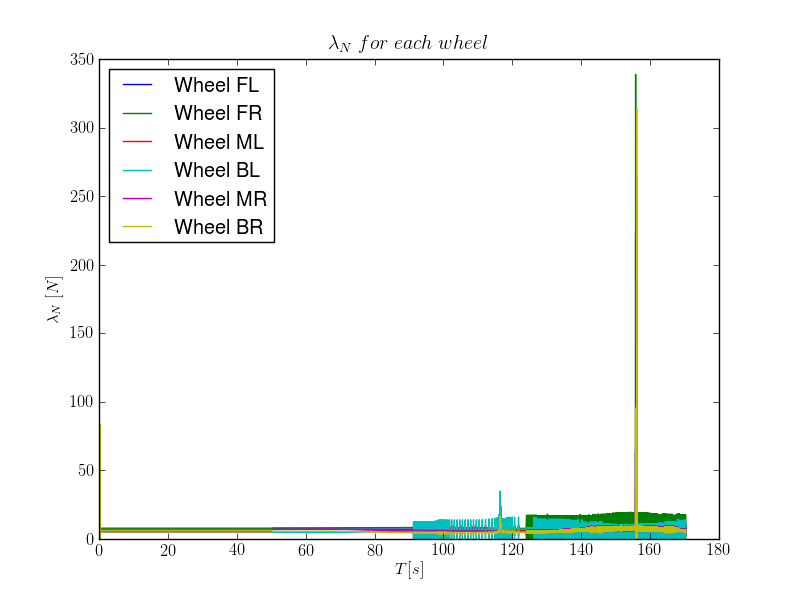
\includegraphics[width=0.8\textwidth]{lambdaN8}
  \caption{$\lambda_N$}
\end{figure}

\begin{itemize}
  \item $\lambda_{T_x}$ - tangential component of the contact force in the x direction for each wheel
\end{itemize}

\begin{figure}[H]
  \centering
    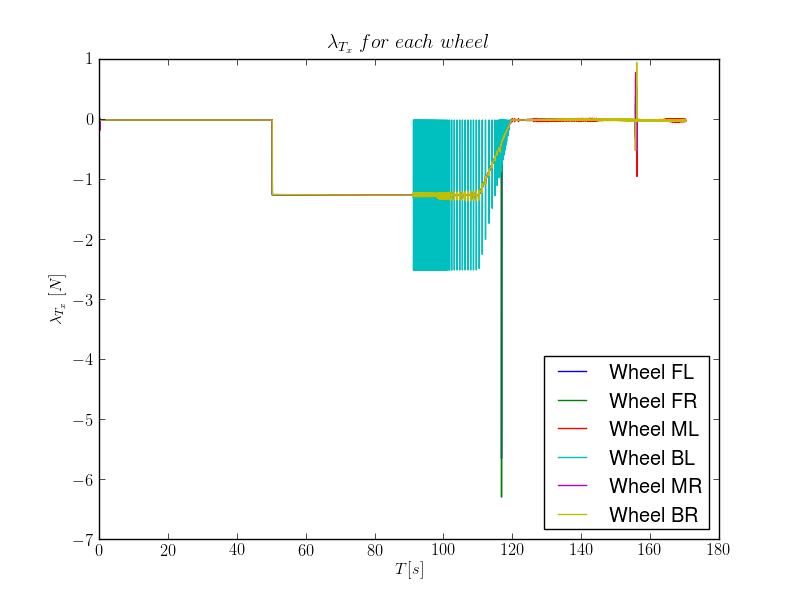
\includegraphics[width=0.8\textwidth]{lambdaTx8}
  \caption{$\lambda_{T_x}$}
\end{figure}

\begin{itemize}
  \item $\lambda_{T_z}$ - tangential component of the contact force in the z direction for each wheel
\end{itemize}

\begin{figure}[H]
  \centering
    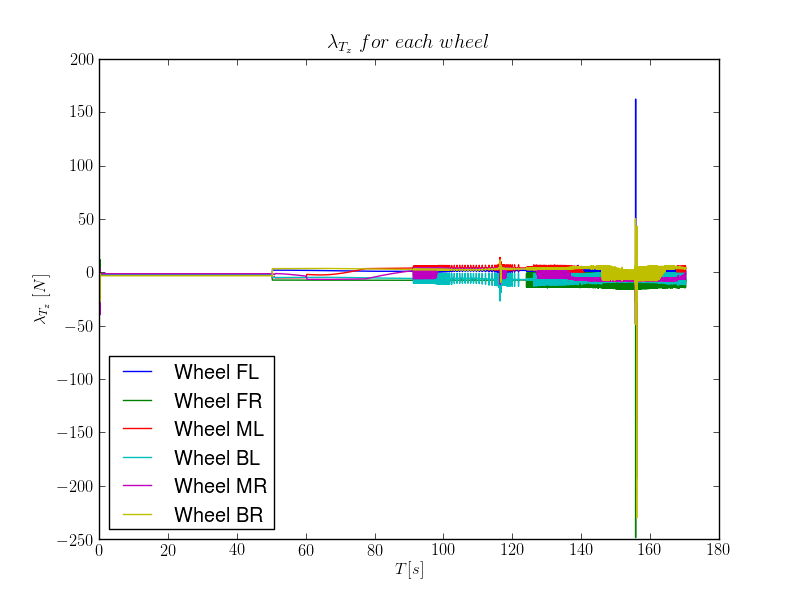
\includegraphics[width=0.8\textwidth]{lambdaTz8}
  \caption{$\lambda_{T_z}$}
\end{figure}

\begin{itemize}
  \item $y_{N}$ - gap function (distance between contact point and the constraint function) for each wheel
\end{itemize}

\begin{figure}[H]
  \centering
    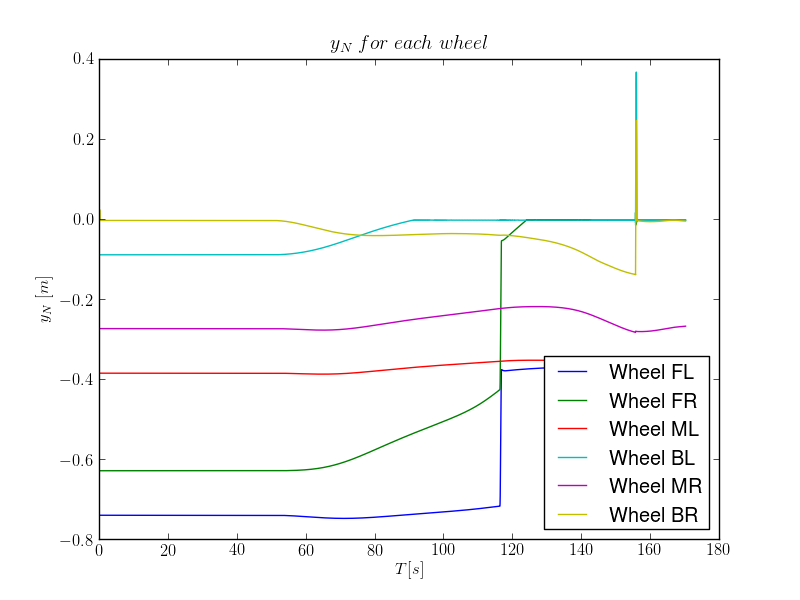
\includegraphics[width=0.8\textwidth]{yN8}
  \caption{$y_N$}
\end{figure}

